\providecommand{\main}{..}
\documentclass[\main/main.tex]{subfiles}

\begin{document}

\lesson{11}{04/11/20}
\section{Non-equilibrium Conditions in a Continuous System}

\textit{\textbf{Summary}}: in the previous lecture we introduced the idea of \textit{generalized response function} in the context of LRT (weak perturbations) $\Xi_{ij}(t)$, which describes the response of observable $i$ to the perturbation provided by the field conjugated to observable $j$. 

What we have shown is that, upon time reversal, we can exchange the two indexes of the response function and what we get is:
\begin{equation}
    \Xi_{ij}(t)=\tau_i\tau_j\Xi_{ji}(t)
\end{equation}
where $\tau_i,\tau_j$ are the eigenvalues of the corresponding observables for the time reversal operator $\mathcal{T}$, $\mathcal{T}X_i=\tau_i X_i$; if $\tau=+1$ the observable is even upon time reversal, if $\tau=-1$ it's odd.

In the simplest case in which our perturbation is just step-wise, as shown in Figure \ref{fig:pert}, then we can deduce the so called \textit{Onsager regression relation}:
\begin{equation}
    \mean{X_i(t)}=\beta h\mean{X_i(t)X_j(0)}_0
    \label{eq:ons}
\end{equation}
The main point is that on the left hand side we have a non-equilibrium average, while on the right hand side we have an equilibrium average of the correlation function between the two different observables. \\

We moved then in the context of \textit{entropy production rate}, where the entropy of the universe can be written as:
\begin{equation}
    d\mathbb{S}=dS+dS_r; \qquad d\mathbb{S}\geq 0
\end{equation}
Our variable $X_i$ is an \textit{extensive thermodynamic observable} and we can define an \textit{affinity} $\mathbb{F}_i$ just deriving the overall entropy with respect to $X_i$, which is the system's observable:
\begin{equation}
    \mathbb{F}_i=\frac{\partial \mathbb{S}}{\partial X_i}=F_i-F_i^{(r)}
\end{equation}
where (-) entropy is a thermodynamic potential for the system that, at equilibrium, takes a minimum (?) value.\\

We can consider an example introducing the so called $(\mu,T,P)$ ensemble in which we allow the exchange of energy, particles and variation in volume with the reservoir: in this case we can compute the entropy change $dS$ as

\begin{equation}
T d S=d U+P d V-\sum_{j} \mu_{j} d N_{j} 
\label{eq:gibbs2}
\end{equation}

where $P$ is the absolute pressure and $\mu_j$ is the chemical potential for the particle subspecies $j$.

The point is that the affinity related to the energy/volume/number of particles of species $j$ ($\mathbb{F}_{U,V,N_j}$, here we are considering energy/volume/number of particles of species $j$ as my extensive observable) then we get that

\begin{equation}
    \mathbb{F}_{U}=\frac{1}{T}-\frac{1}{T_{r}}, \quad \mathbb{F}_{V}=\frac{P}{T}-\frac{P_{r}}{T_{r}}, \quad \mathbb{F}_{N_{j}}=-\frac{\mu_{j}}{T}+\frac{\mu_{j}^{(r)}}{T_{r}}
\end{equation}

At equilibrium  we want affinities to be zero (because we are in the minimum of the entropy and the derivative of entropy with respect to (?) must be zero) and then $(T,P,\mu_j)$ needs to be the same in the system as in the reservoir. \\

Out-of-equilibrium we characterized the situation by using \textit{fluxes}, so the variation in time of the observables we are interested in is expressed as $J_i=dX_i/dt$ and in the end the \textit{entropy production rate} (how the entropy is increasing in time) can be written as
\begin{equation}
    \frac{d\mathbb{S}}{dt}=\sum_i\mathbb{F}_iJ_i\geq 0 \quad \text{for the 2$^{nd}$ law of TD}
    \label{eq:2l}
\end{equation}

\begin{center}
    -------------------------------------------------------------------
\end{center}

Let's now extend the formalism we've presented to the case of \textit{two} reservoir ($a,b$): with $\mathbf{X}_i$ we describe our observable in the universe and it is defined as
\begin{equation}
    \mathbb{X}_i=X_i + X_i^{(a)} + X_i^{(b)}
\end{equation}
We will consider in general our extensible observables which are conserved at least in the universe (e.g. $U,V,N \dots$) which implies that $d\mathbb{X}_i=0=dX_i + dX_i^{(a)} + dX_i^{(b)}$. It's important to point out that the reservoir in general is bigger than the system, so we will assume that we can neglect the variation in the system, $dX_i\simeq 0$ and  so:
\begin{equation}
    d\mathbb{X}_i = 0 = \cancel{dX_i} + dX_i^{(a)} + dX_i^{(b)} \simeq  dX_i^{(a)} + dX_i^{(b)} \implies  dX_i^{(a)} \overset{(*)}{=} - dX_i^{(b)}
\end{equation}
and so the entropy production rate can be written as
\begin{equation}
    \frac{d\mathbb{S}}{dt}\approx \sum_i \left[ \underbrace{\frac{\partial S_a}{ dX_i^{(a)}} - \frac{\partial S_b}{ dX_i^{(b)}}}_{\mathbb{F}_i} \right]J_i^{(a)}
    \label{eq:epr}
\end{equation}
because from (*) we can state that $J_i^{(a)}=-J_i^{(b)}$ and we can express (\ref{eq:epr}) using only one flux. Obviously this is an approximation because we are neglecting what is happening in the system. \\

To make this example more specific let's consider a situation (represented in Figure \ref{fig:res}) with two reservoirs  at different temperatures $T^{(a)},T^{(b)}$ with $T^{(a)}<T^{(b)}$: in this situation the heat flux goes from (b) to (a).

For this reason, considering as unique extensive observable the energy $U$ (which implies that the affinity is $T^{-1}$), the entropy rate can be written as:
\begin{equation}
    \frac{d\mathbb{S}}{dt}\approx\left(\underbrace{\frac{1}{T^{(a)}} - \frac{1}{T^{(b)}}}_{\mathbb{F}_U>0}\right)J_U^{(a)} \overset{(\ref{eq:2l})}{\geq} 0 \implies J_U^{(a)} > 0
\end{equation}

which means that reservoir (a) is absorbing energy (which is correct because is the coldest reservoir) whereas the flux for reservoir (b) is the opposite and it's negative for (*) because it's giving out energy. 

\begin{figure}[ht]
    \centering
    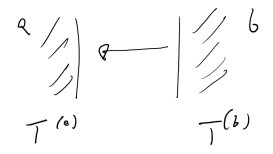
\includegraphics[width=0.65\linewidth]{Lectures/Images/reservoirs.jpg}
    \caption{Example using two reservoirs at different temperatures $T^{(a)},T^{(b)}$, where $T^{(a)}<T^{(b)}$.}
    \label{fig:res}
\end{figure}


How can we generalize then the equation for entropy production rate in the case of continuous systems? \\

So far we have talked about a system referring to it with its energy and about the system as a whole: introducing some space variables in the system we are now allowed to talk about \textit{local energy/entropy density} as a function of the position in the system. We will now deal with entropy and observables functions like $S(\Vec{r});X_i(\Vec{r})$: this is not obvious because when we write entropy as a function of the position we are implicitly assuming \textit{local equilibrium} (as in the context of LRT) but it is not granted at all in general.

Assuming we can talk about local equilibrium and knowing that $F_i=\partial S/\partial X_i$ we can write that (switching from extensive to \textit{intensive} quantities $s:=S/V;x:=X/V$\footnote{Affinities stay the same, $ F_i={\partial s}/{\partial x_i}$.}):
\begin{equation}
    ds=\sum_i F_i dx_i
\end{equation}
A similar relation applies to the corresponding current densities: to entropy density and observable density we can associate a current density $\Vec{j}_s$, namely
\begin{equation}
\Vec{j}_s=\sum_iF_i\Vec{j}_i
    \label{eq:changes}  
\end{equation}

where $\Vec{j}_i$ is the current density for $x_i$ and $\Vec{j}_s$ is the current density for entropy.

The main point is that entropy is not conserved (entropy out-of-equilibrium can increase) and so in a region of a continuous system we can say that the rate of local production of entropy
is given by the entropy entering/leaving this region (surface term) plus the rate of increase 
of entropy within this region (volume term), as
\begin{equation}
    \frac{ds}{dt}=\underbrace{\frac{\partial s}{\partial t}}_{\text{Volume term}} +\,\,\,\underbrace{\Vec{\nabla}\cdot \Vec{j}_s}_{\text{Surface term}}
    \label{eq:entr}
\end{equation}
which is generally not zero because entropy is not conserved.

On the other hand the other observables $x_i$ are conserved and so the overall variation can be written as:
\begin{equation}
    \frac{dx_i}{dt}=\frac{\partial x_{i}}{\partial t}+\Vec{\nabla} \cdot \vec{j}_{i}=0
    \label{eq:var}
\end{equation}

which is the well-known continuity equation. 
The goal now is to write an equation for the entropy production rate.

Considering now the (partial) time derivative of (\ref{eq:changes}):
\begin{equation}
    \frac{\partial s}{\partial t}=\sum_i F_i \frac{\partial x_i}{\partial t}
\end{equation}

while computing the divergence of the entropy current density
\begin{equation}
    \vec{\nabla}\cdot \vec{j}_s\overset{(\ref{eq:entr})}{=}\vec{\nabla}\cdot (\sum_i F_i\vec{j}_i)=\sum_i(\vec{\nabla}F_i\cdot\vec{j}_i+F_i\vec{\nabla}\cdot\vec{j}_i)
\end{equation}

so finally
\begin{equation}
     \frac{ds}{dt}={\frac{\partial s}{\partial t}}+\Vec{\nabla}\cdot \Vec{j}_s = \sum_i F_i \left(\underbrace{\hlc{yellow}{\frac{\partial x_{i}}{\partial t}+\Vec{\nabla} \cdot \vec{j}_{i}}}_{=0}\right)+\sum_i\vec{\nabla}F_i\cdot\vec{j}_i
\end{equation}
where the yellow term is null because $x_i$ is conserved.

In the end the final equation describing the overall entropy production rate for a continuous system is:
\begin{equation}
    \boxed{\frac{ds}{dt}=\sum_i\vec{\nabla}F_i\cdot\vec{j}_i}
    \label{eq:continuos}
\end{equation}

which is the continuous analogue for $dS/dt\overset{(*)}{=}\sum_i\mathbb{F}_iJ_i$, where instead of fluxes we have current densities and we have the gradient of the affinities. \\

The relation with the non-continuos case can be seen in the affinities: in (\ref{eq:continuos}) we can think of them as the difference between the affinities computed into nearby positions ($\vec{\mathbb{F}}_i=\vec{\nabla}F_i(\vec{r})$), while in (*) $\mathbb{F}_i=F_i-F_i^{(r)}$.

\section{Phenomenological equations involving transport kinetic coefficient}
After having identified the affinities, we can proceed to the main goal of the thermodynamics of irreversible processes, i.e., finding a relation between affinities and fluxes. For this
purpose, always in the framework of LRT (weak perturbations), we will introduce two sets of empirical phenomenological coefficients, called $\mathcal{M}_{ij}$ and $L_{ij}$ where the second ones are called \textit{Onsager kinetic coefficients}. \\

We suppose that fluctuating macroscopic observables\footnote{No spatial dependence is assumed.} $X_i(t)$ evolve in time according to linear equations of the form\footnote{Because of the fact that we are dealing with empirical coefficients/relations we are in general dealing also with (\textbf{non-equilibrium}) averages: sometimes they can be omitted, pay attention. Since we are out-of-equilibrium we ha a non-zero current.}
\begin{equation}
\boxed{\mean{J_{i}}=\frac{d}{d t} \mean{X_{i}(t)}:=-\sum_{k} \mathcal{M}_{i k} \mean{X_{k}(t)}}
\label{eq:m}
\end{equation}

So the $\mathcal{M}$ coefficients describe how the time variation of the $X_i$ observable (i.e. the flux $J_i$) is connected to the values of all other observables, including the same observable of course.

In this approach we are describing the coupling between two different observables out-of-equilibrium and we will assume that $\mean{X_i}_0=0$.

In the case of one observable we get that

\begin{equation}
    \frac{d}{d t} \mean{X_{i}(t)}:=-\mathcal{M}_{i i} \mean{X_{k}(t) }\implies \text{exponential decay of} \mean{X_i(t)}
\end{equation}
In other words this diagonal coefficient (if there is no coupling) is telling us how the non-equilibrium average is decaying to the equilibrium value. \\

Using the Onsager regression relation $\mean{X_i(t)} \propto \mean{X_i(t)X_j(0)}_0$ and applying it to equation (\ref{eq:m}) , which defines the $\mathcal{M}$ coefficients, we can replace the non-equilibrium averages on both sides with equilibrium ones:

\begin{equation}
    (\ref{eq:m}) \implies
\frac{d}{d t}\left\langle X_{i}(t) X_{j}(0)\right\rangle_{0}=-\sum_{k} \mathcal{M}_{i k}\left\langle X_{k}(t) X_{j}(0)\right\rangle_0
\label{eq:uso}
\end{equation}
Let's remember that the Onsager regression relation holds in the case of constant perturbation which is then switched off instantaneously at some point. \\

Let's assume now that all our observables are even under time reversal:
\begin{equation}
    \text{If} \,\,\tau_i=\tau_j=1  \implies \mean{X_i(t)X_j(0)}_0=\mean{X_j(t)X_i(t)}_0
    \label{eq:deriva}
\end{equation}
Considering now the time derivative of (\ref{eq:deriva}) for both sides and using (\ref{eq:uso}) we obtain (neglecting the '-' sign at both sides)
\begin{equation}
\sum_{k} \mathcal{M}_{i k}\left\langle X_{k}(t) X_{j}(0)\right\rangle_{0}=\sum_{k} \mathcal{M}_{j k}\left\langle X_{k}(t) X_{i}(0)\right\rangle_{0}
\label{eq:altralabel}
\end{equation}

At this point now we define the Onsager kinetic coefficients $L_{ij}$ such that
\begin{equation}
    L_{ij}=\sum_k\mathcal{M}_{ij}\hlc{yellow}{\mean{X_k X_j}_0}
    \label{eq:lcoeff}
\end{equation}
where the highlighted term is the average of the product of the two observables at the same time, more formally is $\mean{X_k(0) X_j(0)}_0$ and therefore there is time dependence no more.

Evaluating (\ref{eq:altralabel}) at $t=0$ tells us that the matrix of the Onsager coefficients is \textit{symmetric}\footnote{Always assuming that all observables are even under time reversal $\tau_i=\tau_j=1$.}:
\begin{equation}
    L_{ij}=L_{ij}
\end{equation}

Because of the definition given in (\ref{eq:lcoeff}) for the $L_{ij}$ coefficients we can state that the fluxes
\begin{equation}
    \boxed{\mean{J_i}= \frac{d}{dt}\mean{X_i}=\sum_kL_{ik}\mean{\mathbb{F}_k}}
    \label{eq:combined}
\end{equation}

The main difference with the $\mathcal{M}_{ij}$ coefficients in (\ref{eq:m}) is that we express the fluxes as a linear combination of the average of all observables, while the $L_{ij}$ coefficients allow us to write the fluxes as a linear combination of the \textit{affinities} (corresponding to all possible observables). Remember that the previous equation is a phenomenological equation which holds only for weak perturbations; for non LRT we should add $\mathcal{O}(\mathbb{F}^2)$ terms. \\

Actually one can provide a general definition for the Onsager coefficients $L_{ij}$:
\begin{equation}
    L_{i k}=\frac{\partial \mean{J_{i}}}{\partial \mathbb{F}_{j}}\biggr\rvert_{\mathbb{F}_{k}=0\, \forall\,k}
\end{equation}

i.e., the matrix $L$ of the linear kinetic coefficients contains elements that are computed at equilibrium conditions (crucial), i.e., when all affinities $\mathbb{F}_k$ vanish. \\

We will now prove the consistency of the definitions of $\mathcal{M}$ and $L$ starting from (\ref{eq:combined}) and using the previous equation in order to recover (\ref{eq:lcoeff}): using Onsager regression relation we can write (\ref{eq:combined}) such that
\begin{align}
    \frac{d}{dt}\mean{X_i(t)X_j(0)}_0 &=\sum_kL_{ik}\mean{\mathbb{F}_k(t)X_j(0)}_0 \\
    -\sum_k\mathcal{M}_{ik}\mean{X_k(t)X_j(0)}_0 &\overset{(\ref{eq:uso})}{=} 
\end{align}
and changing signs:
\begin{equation}
    \sum_k\mathcal{M}_{ik}\mean{X_k(t)X_j(0)}_0   =-\sum_kL_{ik}\mean{\mathbb{F}_k(t)X_j(0)}_0    
\end{equation}
In the end one can prove that the following average value is\footnote{Proof in the following appendix.}:
\begin{equation}
    \mean{\mathbb{F}_k(t)X_j(0)}_0=-\delta_{kj}
    \label{eq:nome}
\end{equation}
i.e. the correlation equilibrium average of the product of affinity and observable is either $-1$ if $k=j$ of it is zero.

If (\ref{eq:nome}) is true than it implies that we can recover the original definition of $L$ coefficients (\ref{eq:lcoeff}):
\begin{equation}
    \sum_k\mathcal{M}_{ik}\mean{X_kX_j}_0=L_{ij}
\end{equation}

Let's use now equation (\ref{eq:combined}) to go back to the equation for the entropy production rate:
\begin{equation}
    \frac{d \mathbb{S}}{d t}=\sum_iJ_i\mathbb{F}_i=\overset{(\ref{eq:combined})}{=}\sum_{i j} L_{i j} \mathbb{F}_{i} \mathbb{F}_{j}
\end{equation}
which is a \textit{biliniear (quadratic) form} in the affinities $\mathbb{F}_i,\mathbb{F}_j$. This implies that, since from the second law of thermodynamics we know that the entropy production rate needs to be strictly positive ($dS/dt>0$) if we are out-of-equilibrium (i.e. having at least one affinity $\mathbf{\mathbb{F}_i>0}$ for one $i$), the diagonal Onsager coefficients have to be stricly positive $\mathbf{L_{ii}>0}$ and that $\mathbf{det(L)>0}$. \\

From now on we won't use averages but remember that the first line of the previous equation is an exact thermodynamic equation, while the second passage is an empirical phenomenological equation that is true only in the limit of very small perturbation (and so \textbf{very small affinities}\footnote{In our context the thermodynamic quantity which is conjugate to the observable is the affinity.}). \\

We can also compute the time derivative of the entropy production rate (the two factor is due to the fact that we can do this calculation in both ways),
\begin{align}
\frac{d^{2} \mathbb{S}}{d t^{2}} &=2 \sum_{i j} L_{i j} \underbrace{\sum_{k} \frac{\partial \mathbb{F}_{i}}{\partial X_{k}} \overbrace{\frac{d X_{k}}{d t}}^{J_k} }_{d\mathbb{F}_i/dt} \mathbb{F}_{j} = \\
&\overset{(a)}{= }2 \sum_{i k} \frac{\partial \mathbb{F}_{i}}{\partial X_{k}} J_{k} J_{i} =\\
&\overset{(b)}{=}2 \sum_{i k} \frac{\partial^{2} \mathbb{S}}{\partial X_{k} \partial X_{i}} J_{k} J_{i}
\end{align}
where in (a) we used the fact that $L$ is a symmetric matrix and the fact that $J_i=\sum_jL_{ij}\mathbb{F}_j$. We finally remember that $\mathbb{F}=\partial \mathbb{S}/\partial X_i$ in (b).

In this way we can deduce that, since the overall entropy needs to have a maximum at equilibrium (more precisely the entropy $\mathbb{S}(\{X_i\})$ is a concave function of the observables $\{X_i\}$) and this means that the form defined by the second derivatives of the entropy with respect to variables $X_{i},X_{j}$ is a \textit{negative form}.

This implies that 
\begin{align}
    \frac{d^2\mathbb{S}}{dt^2}\leq 0 \implies \frac{d\mathbb{S}}{dt}\quad \text{always decreases}
\end{align}

We can actually deal with two different scenarios: we can have
\begin{itemize}
    \item \textit{relaxation at equilibrium}: asymptotically for infinite time the entropy production rate goes to zero (which is the equilibrium situation) as represented in Figure \ref{fig:e}a;
    \item \textit{relaxation to a stationary non-equilibrium state}: NESS (non-equilibrium steady-state) in which the entropy production rate asymptotically converges to a finite strictly positive value (as represented in Figure \ref{fig:e}b)
\end{itemize}

\begin{figure}[ht]
		\centering
		\subfloat[][\emph{}]
		{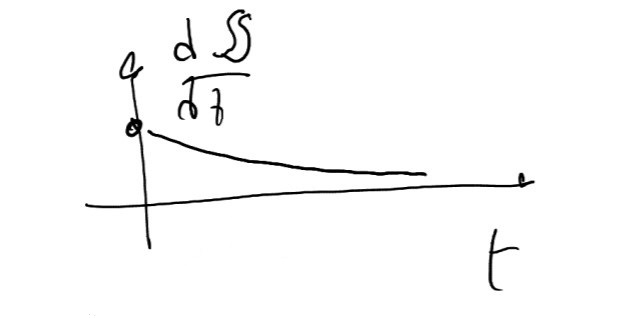
\includegraphics[width=.45\textwidth]{Lectures/Images/Inkede1_LI.jpg}} \quad
		\subfloat[][\emph{}]
		{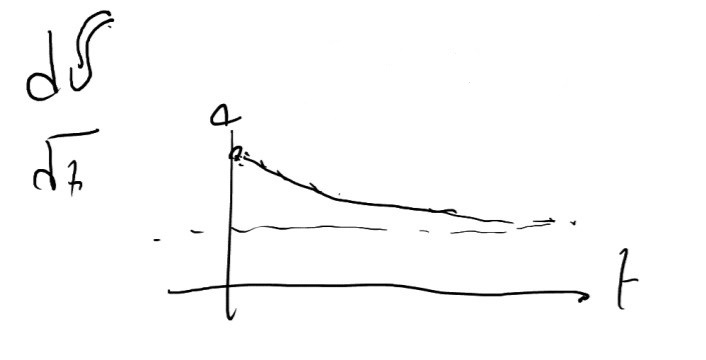
\includegraphics[width=.45\textwidth]{Lectures/Images/Inkede2_LI.jpg}}
		\caption{Graphical representation of EPR in the case of relaxation at equilibrium (a) and NESS (b).}
		\label{fig:e}
	\end{figure}
	
Let us use this formalism to see some examples:
\paragraph{Mechanothermal effect (coupled transport)}

Let's consider a system made of two (fixed) volumes kept at different temperatures $T,T^{(r)}$ containing the
same gas that are in contact through a wall, where a small hole allows for a slow exchange
of particles. The exchanged particles also carry their (internal) energy from one gas to the
other. Energy and particles can be exchanged between the two systems (energy and particles fluxes are involved and they will be \textit{coupled}) and in this sense, this geometry represents the simplest example of coupled transport.

We are dealing with two relevant observables ($U,N$) and the entropy change is defined as
\begin{equation}
    dS=\frac{dU}{T}-\frac{\mu}{T}dN
\end{equation}

The affinities in this simple example are:
$$
\begin{array}{l}
\mathbb{F}_{U}=\frac{1}{T}-\frac{1}{T_{r}} \\
\mathbb{F}_{N}=-\frac{\mu}{T}+\frac{\mu_{r}}{T_{r}}
\end{array}
$$
while the correspondent fluxes are
\begin{equation}
J_{U}=\frac{d U}{d t} \quad \text { and } \quad J_{N}=\frac{d N}{d t}
\end{equation}
Expressing the fluxes using the matrix of the Onsager kinetic coefficients e splitting them in diagonal and off-diagonal contributions we get that 
\begin{equation}
\begin{aligned}
J_{U} &=L_{U U} \mathbb{F}_{U}+L_{U N} \mathbb{F}_{N} \\
J_{N} &=L_{N U} \mathbb{F}_{U}+L_{N N} \mathbb{F}_{N} (*)
\end{aligned}
\end{equation}

(A) Considering the system at \textit{thermal equilibrium} we know that $\mathbb{F}_U=0 (\implies T=T_{r}$ and even at equilibrium we still have a non-zero energy current associated to the number of particles (for $\mathbb{F}_N\neq0$):

\begin{equation}
J_{U}=L_{U N}\left(-\frac{\mu}{T}+\frac{\mu_{r}}{T}\right) 
\end{equation}
the presence of different chemical potentials in the system and in the reservoir the presence of a non-zero off-diagonal Onsager coefficient makes sure that we can find an energy current associated to this situation. For the particles number:
\begin{equation}
    J_{N}=L_{N N}\left(-\frac{\mu}{T}+\frac{\mu_{r}}{T}\right) 
\end{equation}
thus yielding the relation
\begin{equation}
\frac{J_{U}}{J_{N}}=\frac{L_{U N}}{L_{N N}}
\end{equation}

In this situation we have coupled transport of particles and heat by a purely mechanical
effect even in thermal equilibrium conditions. \\

(B) Considering a \textit{thermomechanical effect} we have to deal with a stationary state with zero particle flux $J_N=0$ (we want to archive a zero particle flux and we let just the energy flux survive).

The phenomenological relation (*) reduces to 
\begin{equation}
\frac{\mathbb{F}_{N}}{\mathbb{F}_{U}}=-\frac{L_{U N}}{L_{N N}}; \,\, J_U=\mathbb{F}_U\left[L_{UU}-\frac{L_{UN}^2}{L_{NN}}\right]=\frac{det(L)}{L_{NN}}\mathbb{F}_U
\end{equation}
and in this case we have both affinities that are different  to zero and both of them contributes in driving the system out-of-equilibrium but we are in a special situation in which the particle flux zero (the energy flux is not zero and is determined by both affinities because all the Onsager coefficients contributes to the determinant to establish a non zero energy flux).

Notice also that the ratio between the fluxes in the first case (i.e., the mechanothermal
effect) is equal to minus the ratio of affinities in the second case (i.e., the thermomechanical
effect). This shows that Onsager relations establish interesting phenomenological similarities
among quite different physical phenomena.

\end{document}